\documentclass{article}
\usepackage[margin=1in]{geometry}
\usepackage{pgf}
\usepackage{tikz}
\usetikzlibrary{arrows,automata}
\usepackage[latin1]{inputenc}
\usepackage{listings}
\lstdefinestyle{customc}{
  belowcaptionskip=1\baselineskip,
  breaklines=true,
  frame=L,
  xleftmargin=\parindent,
  language=C,
  showstringspaces=false,
  basicstyle=\footnotesize\ttfamily,
  keywordstyle=\bfseries\color{green!40!black},
  commentstyle=\itshape\color{purple!40!black},
  identifierstyle=\color{blue},
  stringstyle=\color{orange},
}
\lstset{escapechar=@,style=customc}

\begin{document}

\begin{figure}
\center
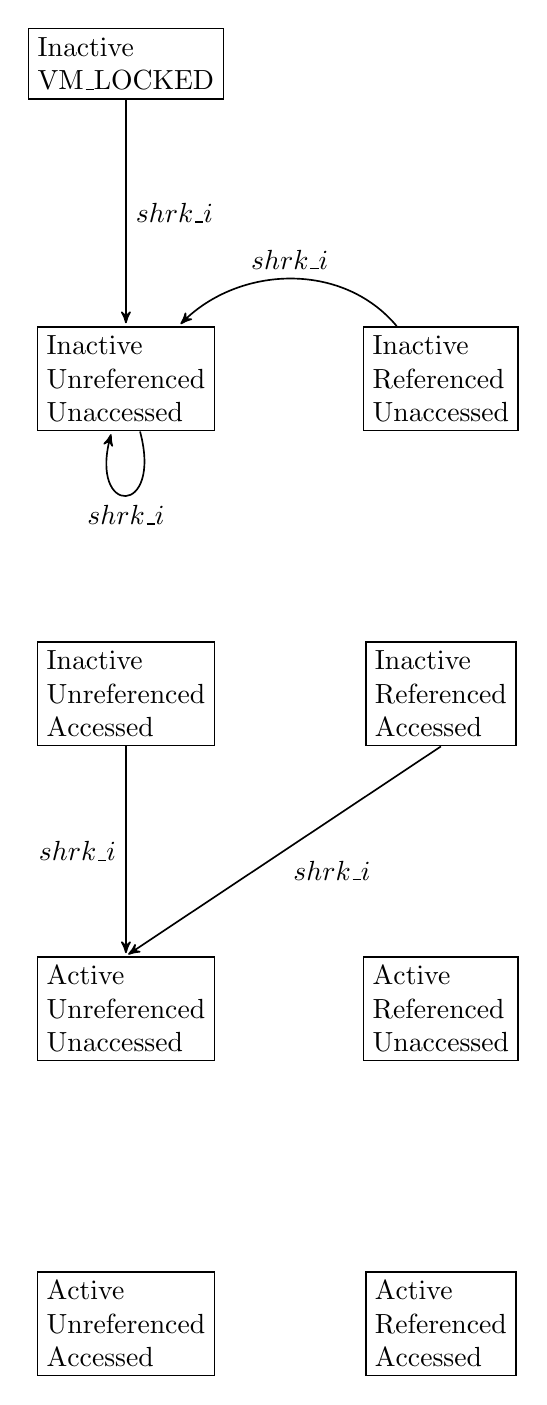
\begin{tikzpicture}[->,>=stealth',shorten >=1pt,auto,node distance=4cm,
                    semithick]

  \tikzstyle{every state}=[rectangle,draw,align=left]

  \node[state] (IUU)                {Inactive \\ Unreferenced \\ Unaccessed};
  \node[state] (IRU) [right of=IUU] {Inactive \\ Referenced   \\ Unaccessed};
  \node[state] (LCK) [above of=IUU] {Inactive \\ VM\_LOCKED};

  \node[state] (IUA) [below of=IUU] {Inactive \\ Unreferenced \\ Accessed  };
  \node[state] (IRA) [right of=IUA] {Inactive \\ Referenced   \\ Accessed  };

  \node[state] (AUU) [below of=IUA] {Active   \\ Unreferenced \\ Unaccessed};
  \node[state] (ARU) [right of=AUU] {Active   \\ Referenced   \\ Unaccessed};

  \node[state] (AUA) [below of=AUU] {Active   \\ Unreferenced \\ Accessed};
  \node[state] (ARA) [right of=AUA] {Active   \\ Referenced   \\ Accessed};

  \path
  (LCK) edge [out=270,in=90,looseness=0]      node {$shrk\_i$} (IUU)
  (IUU) edge [loop below]                     node {$shrk\_i$} (IUU)
  (IRU) edge [out=130,in=45,looseness=1,swap] node {$shrk\_i$} (IUU)

  (IUA) edge [out=270,in=90,looseness=0,swap] node {$shrk\_i$} (AUU)
  (IRA) edge [out=270,in=90,looseness=0]      node {$shrk\_i$} (AUU)
  ;
\end{tikzpicture}
\caption{Anon LRU Automata}
\end{figure}

\begin{figure}
\center
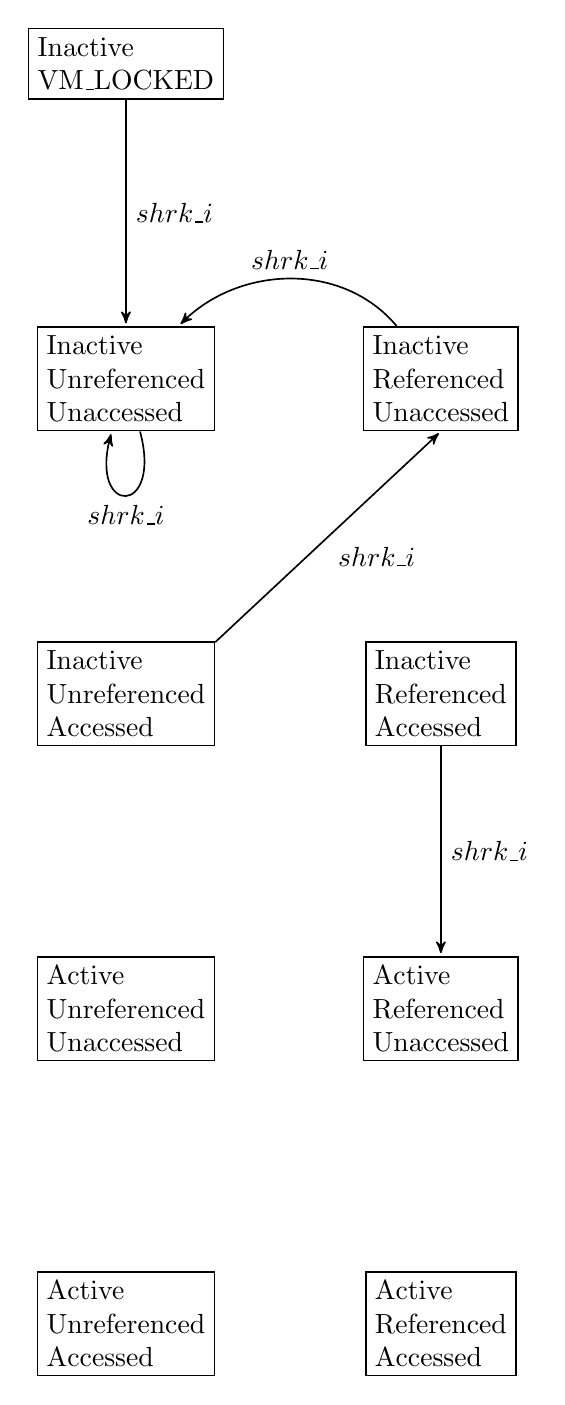
\begin{tikzpicture}[->,>=stealth',shorten >=1pt,auto,node distance=4cm,
                    semithick]

  \tikzstyle{every state}=[rectangle,draw,align=left]

  \node[state] (IUU)                {Inactive \\ Unreferenced \\ Unaccessed};
  \node[state] (IRU) [right of=IUU] {Inactive \\ Referenced   \\ Unaccessed};
  \node[state] (LCK) [above of=IUU] {Inactive \\ VM\_LOCKED};

  \node[state] (IUA) [below of=IUU] {Inactive \\ Unreferenced \\ Accessed  };
  \node[state] (IRA) [right of=IUA] {Inactive \\ Referenced   \\ Accessed  };

  \node[state] (AUU) [below of=IUA] {Active   \\ Unreferenced \\ Unaccessed};
  \node[state] (ARU) [right of=AUU] {Active   \\ Referenced   \\ Unaccessed};

  \node[state] (AUA) [below of=AUU] {Active   \\ Unreferenced \\ Accessed};
  \node[state] (ARA) [right of=AUA] {Active   \\ Referenced   \\ Accessed};

  \path
  (LCK) edge [out=270,in=90,looseness=0]      node {$shrk\_i$} (IUU)
  (IUU) edge [loop below]                     node {$shrk\_i$} (IUU)
  (IRU) edge [out=130,in=45,looseness=1,swap] node {$shrk\_i$} (IUU)

  (IUA) edge [in=270,out=30,looseness=0,swap] node {$shrk\_i$} (IRU)
  (IRA) edge [out=270,in=90,looseness=0]      node {$shrk\_i$} (ARU)
  ;
\end{tikzpicture}
\caption{File LRU Automata}
\end{figure}

\begin{figure}
\center
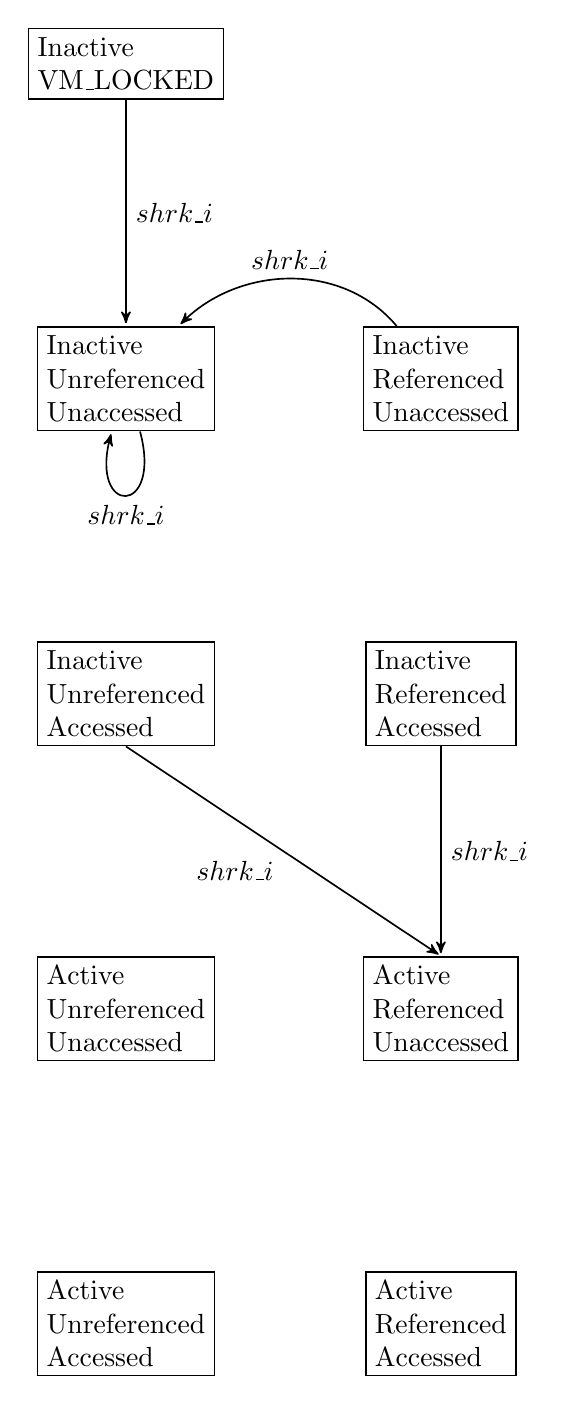
\begin{tikzpicture}[->,>=stealth',shorten >=1pt,auto,node distance=4cm,
                    semithick]

  \tikzstyle{every state}=[rectangle,draw,align=left]

  \node[state] (IUU)                {Inactive \\ Unreferenced \\ Unaccessed};
  \node[state] (IRU) [right of=IUU] {Inactive \\ Referenced   \\ Unaccessed};
  \node[state] (LCK) [above of=IUU] {Inactive \\ VM\_LOCKED};

  \node[state] (IUA) [below of=IUU] {Inactive \\ Unreferenced \\ Accessed  };
  \node[state] (IRA) [right of=IUA] {Inactive \\ Referenced   \\ Accessed  };

  \node[state] (AUU) [below of=IUA] {Active   \\ Unreferenced \\ Unaccessed};
  \node[state] (ARU) [right of=AUU] {Active   \\ Referenced   \\ Unaccessed};

  \node[state] (AUA) [below of=AUU] {Active   \\ Unreferenced \\ Accessed};
  \node[state] (ARA) [right of=AUA] {Active   \\ Referenced   \\ Accessed};

  \path
  (LCK) edge [out=270,in=90,looseness=0]      node {$shrk\_i$} (IUU)
  (IUU) edge [loop below]                     node {$shrk\_i$} (IUU)
  (IRU) edge [out=130,in=45,looseness=1,swap] node {$shrk\_i$} (IUU)

  (IRA) edge [out=270,in=90,looseness=0]      node {$shrk\_i$} (ARU)

  (IUA) edge [in=90,out=270,looseness=0,swap] node {$shrk\_i$} (ARU)
  ;
\end{tikzpicture}
\caption{VM\_EXEC File LRU Automata}
\end{figure}

\begin{figure}
\center
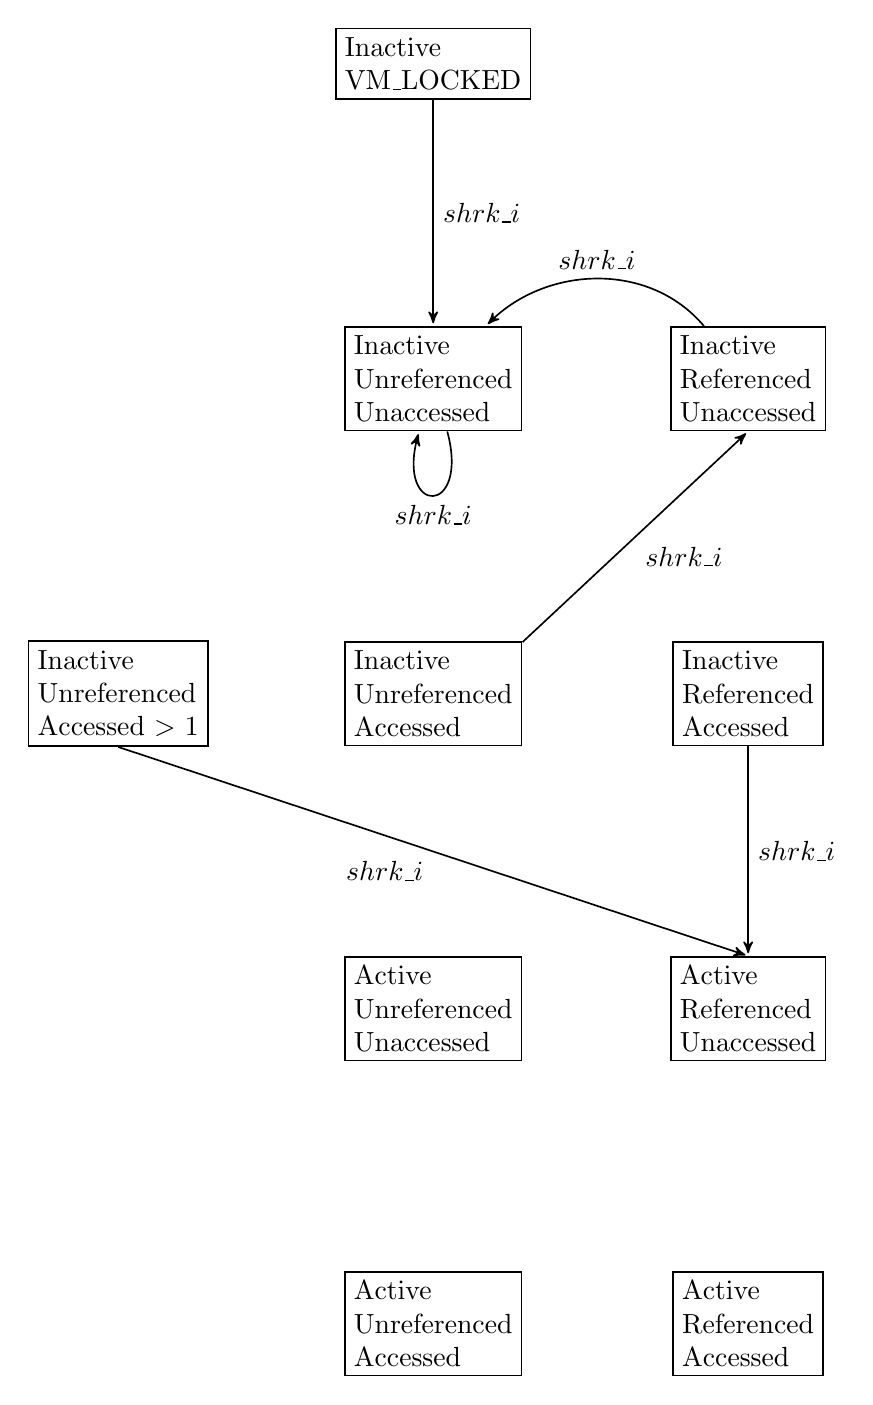
\begin{tikzpicture}[->,>=stealth',shorten >=1pt,auto,node distance=4cm,
                    semithick]

  \tikzstyle{every state}=[rectangle,draw,align=left]

  \node[state] (IUU)                {Inactive \\ Unreferenced \\ Unaccessed};
  \node[state] (IRU) [right of=IUU] {Inactive \\ Referenced   \\ Unaccessed};
  \node[state] (LCK) [above of=IUU] {Inactive \\ VM\_LOCKED};

  \node[state] (IUA) [below of=IUU] {Inactive \\ Unreferenced \\ Accessed};
  \node[state] (IRA) [right of=IUA] {Inactive \\ Referenced   \\ Accessed};
  \node[state] (IAA) [left  of=IUA] {Inactive \\ Unreferenced \\ Accessed $>$ 1};

  \node[state] (AUU) [below of=IUA] {Active   \\ Unreferenced \\ Unaccessed};
  \node[state] (ARU) [right of=AUU] {Active   \\ Referenced   \\ Unaccessed};

  \node[state] (AUA) [below of=AUU] {Active   \\ Unreferenced \\ Accessed};
  \node[state] (ARA) [right of=AUA] {Active   \\ Referenced   \\ Accessed};

  \path
  (LCK) edge [out=270,in=90,looseness=0]      node {$shrk\_i$} (IUU)
  (IUU) edge [loop below]                     node {$shrk\_i$} (IUU)
  (IRU) edge [out=130,in=45,looseness=1,swap] node {$shrk\_i$} (IUU)

  (IUA) edge [in=270,out=30,looseness=0,swap] node {$shrk\_i$} (IRU)
  (IRA) edge [out=270,in=90,looseness=0]      node {$shrk\_i$} (ARU)

  (IAA) edge [in=90,out=270,looseness=0,swap] node {$shrk\_i$} (ARU)
  ;
\end{tikzpicture}
\caption{Shmem LRU Automata}
\end{figure}

\end{document}
